\chapter{Metody lokalizacji na podstawie znaczników radiowych}
\label{ch:metody-lokalizacji}

Znaczniki radiowe, rozmieszczone w ustalonych miejscach środowiska pracy robota, pozwalają na podjęcie zadania lokalizacji na kilka różnych sposobów. W niniejszym rozdziale przedstawiono podstawowe metody lokalizacji.

\section{Fingerprinting}
Metoda fingerprintingu (ang.\textit{fingerprint} - odcisk palca) opiera się na zbiorze punktów referencyjnych. Punkty referencyjne zbiera się w fazie off-line, zapisując w bazie danych położenie danego punktu w przestrzeni oraz referencyjny wektor RSSI postaci $P_{ref} = [ P_{ref \ 1} \cdots P_{ref  \ N}]$, gdzie $N$ jest liczbą znaczników w środowisku, zaś $P_{ref \ i}$ oznacza siłę sygnału RSSI z $i$-tego znacznika \cite{fingerprinting}. Przykładowe rozmieszczenie znaczników i punktów referencyjnych pokazuje schemat na rys. \ref{fig:fingerprinting}.


\begin{figure}[H]
\centering
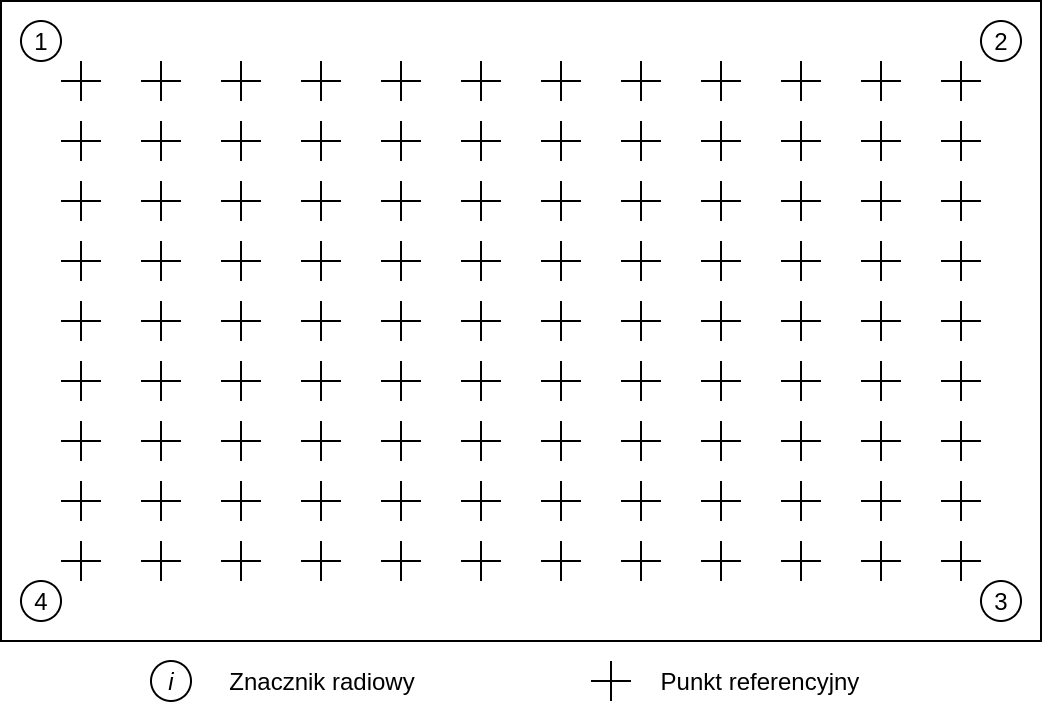
\includegraphics[width=0.7\textwidth]{img/fingerprinting.png}
\caption{Rozmieszczenie znaczników radiowych i punktów referencyjnych w metodzie fingerprintingu. Znaczniki radiowe oznaczono kółkami z cyfrą, punkty referencyjne }
\label{fig:fingerprinting}
\end{figure}

W fazie on-line lokalizowany odbiornik rejestruje wektor siły sygnału $P = [ P_{RX \ 1} \cdots P_{RX \ n}]$ dla danego położenia, następnie obliczana jest odległość wektora $P$ od wektorów referencyjnych $P_{ref}$ według metryki euklidesowej \cite{fingerprinting2}:


\begin{equation}
\label{eq:fingerprinting_odleglosc}
 D(Z, Z_i) = \sqrt{\sum_{j=1}^{N} (P_{ref \ i \ j}-P_{RX \ j})^2}.
\end{equation}

Z odległością \ref{eq:fingerprinting_odleglosc} jako kryterium, można wyszukać K najbliższych sąsiadów wektora $P_{RX}$ w zbiorze punktów referencyjnych $P_{ref}$. Publikacja \cite{fingerprinting2} proponuje następujące podejścia:
\begin{enumerate}
 \item $K = 1$ - za wynik lokalizacji przyjmowany jest najbliższy punkt referencyjny,
 \item $K > 1$ - za wynik lokalizacji przyjmowany jest środek ciężkości najbliższych $K$ punktów referencyjnych.
\end{enumerate}

Wyszukiwanie sąsiadów można prowadzić na pełnym zbiorze punktów referencyjnych lub tylko na jego części, ograniczonej np. do pewnego promienia wokół poprzedniej pozycji. Pozwala to na przyspieszenie wyszukiwania \cite{fingerprinting}. Jakość lokalizacji można dodatkowo poprawić wykorzystując metody probabilistyczne takie jak filtr Bayesa lub cząsteczkowy \cite{fingerprinting2}.

Niewątpliwą zaletą lokalizacji w oparciu o fingerprinting jest to, iż uwzględnia ona nieizotropowy rozkład siły sygnału RSSI w zależności od położenia odbiornika. Ponadto nie jest konieczne wyznaczanie modelu propagacji radiowej do przeliczania RSSI na odległość. Jeśli siatka punktów referencyjnych jest odpowiednio gęsta, fingerprinting jest w stanie zapewnić zadowalające rezultaty. Z drugiej strony, lokalizacja tą metodą wymaga przeprowadzenia dość złożonej kalibracji w fazie off-line (budowanie zbioru punktów referencyjnych), ponadto konieczne jest zapewnienie metody wydajnego przeszukiwania zbioru referencyjnego, zaś jeśli zbiór ten zawiera mało punktów, jakość lokalizacji może być niezadowalająca. 


\section{Trilateracja}
\label{sec:trilateracja}
Trilateracja, obok triangulacji, jest jedną z metod geometrycznych wyznaczania położenia obiektu za pomocą pomiaru kąta lub odległości względem ustalonego węzła. Triangulacja opiera się na pomiarze kątów, natomiast trilateracja - odległości. Dzięki temu możliwe jest zastosowanie jej w lokalizacji w oparciu o pomiar siły sygnału RSSI, związanej z odległością. 

Zadanie trilateracji polega na wyznaczeniu położenia lokalizowanego obiektu, znając odległości tego obiektu od 3 (przypadek dwuwymiarowy) lub 4 (przypadek trójwymiarowy) punktów referencyjnych o znanym położeniu. W dalszej części pracy rozważany będzie tylko przypadek dwuwymiarowy. Oznaczmy $i$-ty punkt referencyjny przez $O_i(x_i, y_i)$. Odległość punktu referencyjnego od lokalizowanego obiektu znajdującego się w punkcie $P(x,y)$ wynosi $R_i$ (rys. \ref{fig:trilateracja-ideal}). O ile punkty $O_i$ nie są współliniowe, punkt $P$ znajduje się na przecięciu okręgów $(O_1, R_1)$, $(O_2, R_2)$, $(O_3, R_3)$. Dlatego rozwiązanie zadania trilateracji można zapisać następująco \cite{trilat_przeglad}:

\begin{equation}
\label{eq:trilateracja1}
 (x - x_1)^2 + (y-y_1)^2 = R_1^2
\end{equation}
\begin{equation}
 (x - x_2)^2 + (y-y_2)^2 = R_2^2
\end{equation}
\begin{equation}
\label{eq:trilateracja3}
 (x - x_3)^2 + (y-y_3)^2 = R_3^2
\end{equation}

Jest to układ równań nieliniowych. Ponieważ liczba punktów referencyjnych może być większa od 3, możemy mieć do czynienia z układem nadokreślonym. Do rozwiązania takiego układu można wykorzystać metodę macierzy pseudo-odwrotnych \cite{trilat_particle}. Generalnie, analityczne rozwiązanie takiego układu równań przedstawia znaczne trudności lub jest niemożliwe \cite{trilat_przeglad}, natomiast rozwązanie numeryczne jest obarczone znacznym błędem \cite{trilat_particle}. Ponadto, w realistycznym przypadku, okręgi nie będą przecinać się w jednym punkcie. Możliwe jest, że będzie więcej punktów przecięcia (rys. \ref{fig:trilateracja-real1}) lub okręgi nie będą się przecinać (rys. \ref{fig:trilateracja-real2}). W obu tych przypadkach powyższy układ równań nie będzie miał rozwiązań. 


\begin{figure}[h]
\centering
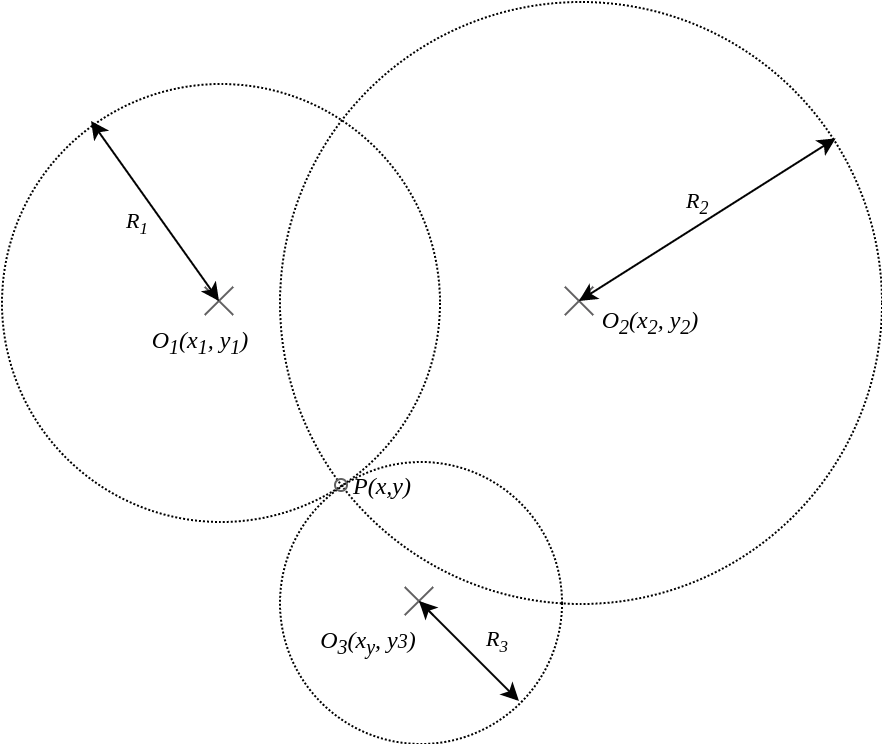
\includegraphics[width=0.6\textwidth]{img/trilateracja-okregi1.png}
\caption{Trilateracja - przypadek idealny}
\label{fig:trilateracja-ideal}
\end{figure}

\begin{figure}[h]
\centering
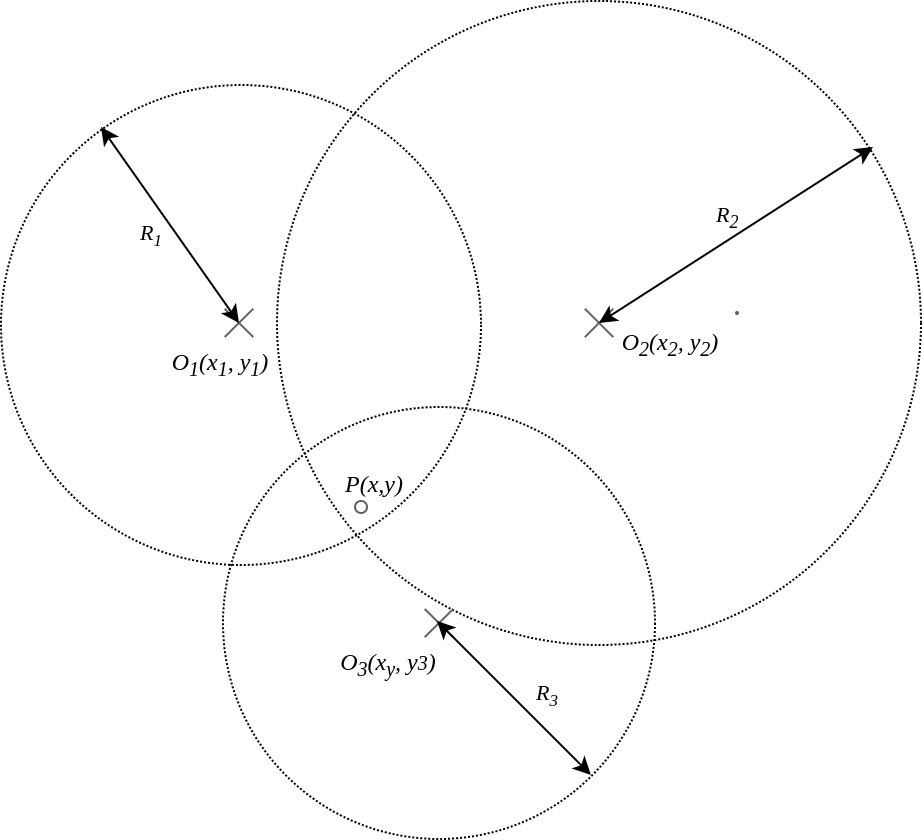
\includegraphics[width=0.6\textwidth]{img/trilateracja-okregi2.png}
\caption{Trilateracja - przypadek rzeczywisty - okręgi nakładają się}
\label{fig:trilateracja-real1}
\end{figure}

\begin{figure}[h]
\centering
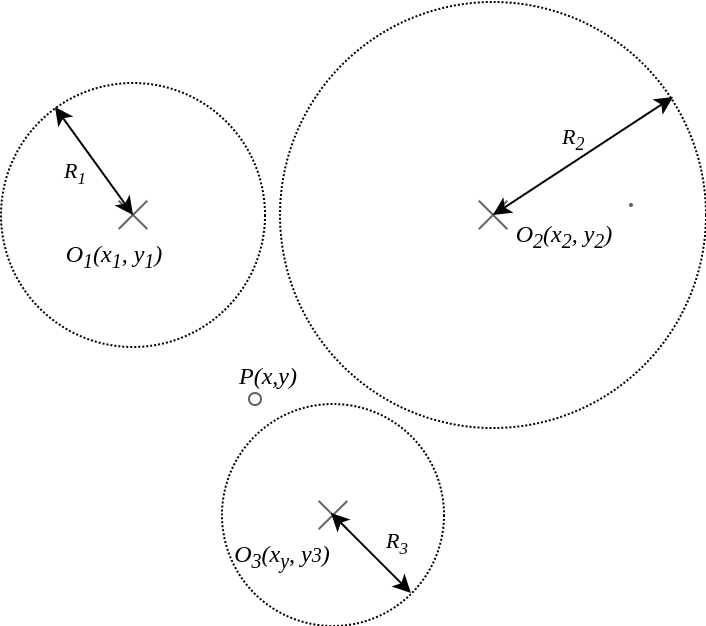
\includegraphics[width=0.6\textwidth]{img/trilateracja-okregi3.png}
\caption{Trilateracja - przypadek rzeczywisty - okręgi wogóle się nie przecinają}
\label{fig:trilateracja-real2}
\end{figure}


W celu osiągnięcia dobrego rozwiązania numerycznego zadania trilateracji, można posłużyć się algorytmem iteracyjnym \cite{trilat_iter}. Algorytm wymaga, żeby znane były położenia co najmniej 3 punktów referencyjnych $(x_i, y_i)$, oraz zmierzone odległości lokalizowanego obiektu od tych punktów $R_i$, oraz początkowa estymata rozwiązania $(x_e, y_e)$. W każdej iteracji obliczana jest różnica między zmierzoną, a estymowaną odległością obiektu od każdego punktu referencyjnego:

\begin{equation}
\label{eq:trilateracja_iter_f}
f_i = | d_i - \sqrt{(x_i - x_e)^2 + (y_i-y_e)^2}|
\end{equation}


Oznaczając przez $\vec R_ {k}$ estymatę rozwiązania w $k$-tej iteracji:
\begin{equation}
\vec R_ {k} = \left( \begin{array}{c} 
x_{e} \\
y_{e} \\
\end{array} \right)
\end{equation}

i posługując się metodą Newtona \cite{trilat_przeglad} możemy przedstawić równanie następnej iteracji:

\begin{equation}
\label{eq:trilateracja_iter}
\vec R_ {k+1} = \vec R_ {k} - (\mathbf{J}_{k}^T \mathbf{J}_{k})^{-1} \mathbf{J}_{k}^T \vec f_{k}
\end{equation}

gdzie:

\begin{equation}
\label{eq:f_wektor}
\vec f_{k} = \left( \begin{array}{c} 
f_{1} \\
f_{2} \\
\vdots \\
f_{n} \\
\end{array} \right) ,
\end{equation}

zaś przez $\mathbf{J}_{k}$ oznaczamy macierz Jakobiego funkcji $f$:

\begin{equation}
\label{eq:J_wektor}
\mathbf{J}_{k} = 
\left( \begin{array}{cc} 
  \frac{\partial f_{1} }{\partial x} & \frac{\partial f_{1} }{\partial y} \\
  \frac{\partial f_{2} }{\partial x} & \frac{\partial f_{2} }{\partial y} \\
  \vdots & \vdots \\	
  \frac{\partial f_{n} }{\partial x} & \frac{\partial f_{n} }{\partial y} \\
\end{array} \right) = 
\left( \begin{array}{cc} 
  \frac{(x_1 - x_e) }{\sqrt{(x_i - x_e)^2 + (y_i-y_e)^2}} & \frac{(y_1 - y_e) }{\sqrt{(x_i - x_e)^2 + (y_i-y_e)^2}} \\
  \frac{(x_2 - x_e) }{\sqrt{(x_i - x_e)^2 + (y_i-y_e)^2}} & \frac{(y_2 - y_e)  }{\sqrt{(x_i - x_e)^2 + (y_i-y_e)^2}} \\
  \vdots & \vdots \\	
  \frac{(x_3 - x_e)}{\sqrt{(x_i - x_e)^2 + (y_i-y_e)^2}} & \frac{(y_n - y_e)  }{\sqrt{(x_i - x_e)^2 + (y_i-y_e)^2}} \\
\end{array} \right).
\end{equation}

Aby wyznaczyć rozwiązanie zadania trilateracji, należy wykonywać kolejne iteracje metody Newtona zgodnie z równaniem \ref{eq:trilateracja_iter}. Jako estymatę początkową można przyjąć np. rozwiązanie zlinearyzowanego układu równań \ref{eq:trilateracja1} - \ref{eq:trilateracja3}.

W porównaniu do fingerprintingu, trilateracja nie wymaga złożonej fazy off-line. Z drugiej strony, jeśli do pomiaru odległości wykorzystywana jest siła sygnału RSSI, pomiar jest obarczony wszystkimi błędami opisanymi w rozdziale \ref{ch:radio}, w szczególności nie ma możliwości, aby uwzględnić nieizotropowy rozkład siły sygnału w pomieszczeniu. 

\section{Filtr cząsteczkowy}
\label{sec:filtr-czasteczkowy}
Filtr cząsteczkowy, należący do metod Monte Carlo, jest bardzo popularnym narzędziem w robotyce mobilnej. Jest to nieparametryczny, quasi-bayesowski filtr probabilistyczny, pozwalający na reprezentowanie stanu robota w postaci funkcji gęstości prawdopodobieństwa, radzący sobie z nie-gaussowskimi i nieliniowymi modelami pomiaru. Poniżej przedstawiono podstawy teorii filtrów cząsteczkowych oraz możliwe zastosowanie w lokalizacji na podstawie odległości od znaczników radiowych. 

W filtrze cząsteczkowym stan robota jest traktowany jako zmienna losowa $x \in X$. Dla robota poruszającego się na płaszczyźnie lokalizacja opisywana jest przez trzy współrzędne:  $ x = (x, y, \theta)$, gdzie $x$, $y$ są współrzędnymi pojazdu w układze współrzędnych związanym z środowiskiem pracy, zaś $\theta$ jest orientacją robota w tym układzie. Rozkład gęstości prawdopodobieństwa położenia robota $p(x_k | z_k)$ w chwili $k$  jest reprezentowany przez dyskretny zbiór $N_p$ cząsteczek, z których każda reprezentuje hipotezę na temat położenia robota $x_i$ oraz przypisaną jej wagę $w_i$, opisującą stopień potwierdzenia tej hipotezy \cite{preskrypt}, \cite{probabilistic_robotics}:

\begin{equation}
 \label{eq:pf_sk}
 S_{k} = \{ x_i, w_i \}, i = 0, 1, \cdots, N_p, 0 \leq w_i \leq 1,
\end{equation}

Algorytm filtra cząsteczkowego składa się z kilku etapów: 
\begin{enumerate}
 \item \textit{Faza predykcji.} Obliczany jest rozkład gęstości a posteriori w chwili $k$:  $p(x_{k} | x_{k-1}, u_{k-1})$ na podstawie rozkładu gęstości prawdopodobieństwa położenia robota w chwili poprzedniej $p(x_{k-1} | z_{k-1})$ oraz wektora sterowań $u_{k-1}$. Uwzględniany jest model ruchu robota -najczęściej wykorzystywane są sensory odometryczne. Akcja sterowania $u_{k-1} $ jest aplikowana dla każdej cząsteczki ze zbioru $S_{k-1}$. W wyniku powyższej operacji otrzymujemy uaktualniony zbiór cząsteczek:
 \begin{equation}
 \label{eq:pf_sk2}
 S'_{k} = \{ x'_i, w'_i \}, i = 0, 1, \cdots, N_p.
\end{equation}

\item \textit{Pomiar.} Na podstawie pomiaru każdej cząsteczce ze zbioru $S'_{k}$ przypisywana jest nowa waga $w_i$. Wagi są wyznaczane na podstawie rozkładu gęstości prawdopodobieństwa pomiaru: $p(z_{k} | x_{k} )$. Wynikiem jest nowy zbiór $S_{k}$, którego wagi są normalizowane:
\begin{equation}
 w_i = \frac{w_i}{\sum_{j=1}^{N_p} w_j}
\end{equation}

Wagi cząsteczek w nowym zbiorze $S_{k}$ estymują rozkład gęstości prawdopodobieństwa położenia robota $p(x_{k} | z_{k})$.

\item \textit{Resampling}. Po kilku iteracjach wg. punktów 1 i 2, większość cząsteczek miała by pomijalnie małe wagi, przez co estymacja gęstości prawdopodobieństwa $p(x_{k} | z_{k})$ byłaby mało dokładna (estymowana małą ilością cząsteczek). Stąd konieczność dokonania resamplingu cząsteczek (ang. ponowne próbkowanie). Cząsteczki o największych wartościach wag $w_i$ są powielane w zbiorze, natomiast cząsteczki o małych wagach są usuwane ze zbioru \cite{preskrypt}. Resampling jest zagadnieniem złożonym i istnieje kilka różnych algorytmów do wykonania tego zadania \cite{trilat_particle}, \cite{particle_pl}.

\item \textit{Wyznaczenie położenia robota.} Na podstawie zbioru cząsteczek $S_{k}$ należy wyznaczyć położenie robota, będące wynikiem działania filtra. Jako położenie robota można przyjąć położenie reprezentowane przez cząsteczkę o największej wadze, lub średnią ważoną cząsteczek (lub średnią ważoną cząsteczek w pewnym otoczeniu cząsteczki o największej wadze) \cite{preskrypt}:

\begin{equation}
 x_{k} = \sum_{j=0}^{N_p} w_j \cdot x_j
\end{equation}

\end{enumerate}

\subsection{Filtr cząsteczkowy dla robota wyposażonego w sensor odometryczny i system pomiaru odległości od znaczników}
Rozważmy robota o napędzie różnicowym, wyposażonego w sensory odometryczne oraz system wyznaczania odległości od znaczników znajdujących się w ustalonych miejscach środowiska pracy robota, np. system działający w oparciu o znaczniki radiowe. Stan robota jest opisywany przez wektor $x$ postaci:

\begin{equation}
\label{eq:x_wektor}
x_{k} = \left( \begin{array}{c} 
x \\
y \\
\theta \\
\end{array} \right) 
\end{equation}.

\subsubsection{Model ruchu}

Ruch robota, rozumiany jako względna różnica dwóch położeń $x_{k-1} = (x \ y \ \theta)^T$ oraz $x_k = (x' \ y' \ \theta')^T$, może być zamodelowany jako złożenie trzech ruchów prostych: obrotu o kąt  $\delta_{rot1}$, przemieszczenia prostoliniowego o długość $\delta_{trans}$ oraz obrotu o kąt $\delta_{rot2}$. Mając dane dwa wektory położenia robota, $x_{k-1}$ oraz $x_k$, parametry tych ruchów prostych można wyznaczyć następująco \cite{probabilistic_robotics}:
\begin{equation}
 \delta_{rot1} = \mathrm{atan2} (y' - y, x'-x) - \theta,
\end{equation}
\begin{equation}
 \delta_{trans} = \sqrt{(x-x')^2+(y-y')^2},
\end{equation}
\begin{equation}
 \delta_{rot2} = \theta' - \theta - \delta_{rot1}.
\end{equation}
Aby uwzględnić błąd wyznaczenia przemieszczenia, należy uwzględnić szum pomiarowy $\varepsilon_b$ o rozkładzie normalnym, zerowej wartości średniej i wariancji $b$:
\begin{equation}
 \hat \delta_{rot1} = \delta_{rot1} - \varepsilon_{\alpha_1 |\delta_{rot1}|+\alpha_2 |\delta_{trans}|},
\end{equation}
\begin{equation}
 \hat \delta_{trans} = \delta_{trans} - \varepsilon_{\alpha_3 |\delta_{trans}|+\alpha_4 |\delta_{rot1} + \delta_{rot2}|},
\end{equation}
\begin{equation}
 \hat \delta_{rot2} = \delta_{rot2} - \varepsilon_{\alpha_1 |\delta_{rot2}|+\alpha_2 |\delta_{trans}|}.
\end{equation}
Parametry $\alpha_1, \cdots, \alpha_4$ są zależne od budowy robota.

Ostatecznie, równanie uaktualnienia ze stanu $x_{k-1}$ do stanu $x_{k}$ wygląda następująco \cite{probabilistic_robotics}:
\begin{equation}
\label{eq:particle_update}
x_{k} = \left( \begin{array}{c} 
x' \\
y' \\
\theta' \\
\end{array} \right) = \left( \begin{array}{c} 
x \\
y \\
\theta \\
\end{array} \right) + \left( \begin{array}{c} 
\hat \delta_{trans} \cos (\theta + \hat \delta_{rot1}) \\
\hat \delta_{trans} \sin (\theta + \hat \delta_{rot1}) \\
\theta + \hat \delta_{rot1} \hat \delta_{rot2} \\
\end{array} \right)
\end{equation}
To równanie jest używane do predykcji stanu robota w kroku 1 algorytmu filtra cząsteczowego. 

\subsubsection{Model pomiaru}
Zadaniem modelu pomiaru w lokalizacji Monte Carlo jest estymowanie rozkładu gęstości prawdopodobieństwa położenia robota na podstawie mapy otoczenia i pomiarów. Zakładamy, że w otoczeniu robota znajdują się znaczniki (ang. \textit{landmarks}) które można jednoznacznie rozróżnić, zaś ich położenie na mapie jest dokładnie znane. Znacznik taki jest opisywany przez trójkę $(x, y, b)$, gdzie $x, y$ to położenie znacznika w środowisku pracy robota, zaś $b$ jest unikalną wartością dyskretną, identyfikującą znacznik. Mapa środowiska robota jest wtedy wektorem \cite{landmarks}:
\begin{equation}
 M = (m_1,  ..., m_n) = \left( 
  \left( \begin{array}{c} 
x_1 \\
y_1 \\
b_1 \\
\end{array} \right),
\cdots,
  \left( \begin{array}{c} 
x_n \\
y_n \\
b_n \\
\end{array} \right)
\right)
\end{equation}
Obserwowany znacznik jest nazywany cechą (ang. \textit{feature}) i jest reprezentowany przez parę $(r, b)$, gdzie $r$ jest zmierzoną odległością od znacznika, zaś $b$ jego identyfikatorem. W danej chwili czasu $k$ pomiar opisywany przez wektor obserwowanych cech \cite{landmarks}:
\begin{equation}
 f(z) = (f_1,  ..., f_n) = \left( 
  \left( \begin{array}{c} 
r_1 \\
b_1 \\
\end{array} \right),
  \left( \begin{array}{c} 
r_2 \\
b_2 \\
\end{array} \right),
\cdots
\right)
\end{equation}
Każda z cech odnosi się do konkretnego znacznika. Wprowadźmy funkcję dopasowującą, która na podstawie cechy i mapy przypisuje cechę do znacznika: $c(f_i, M)$. W rozpatrywanym przypadku, funkcja dopasowująca odnajduje znacznik na podstawie jego identyfikatora $b$. Następnie wyznaczmy odległość (euklidesową) pomiędzy hipoteczną pozycją robota $\hat p$ a zaobserwowanym znacznikiem $m$:
\begin{equation}
 \label{eq:hatri}
 \hat r_i = \sqrt{(m_x - \hat p_x)^2 + (m_y - \hat p_y)^2}
\end{equation}
oraz różnicę międy zmierzoną odległością od znacznika, a odległością wynikłą z hipotetycznej pozycji $\hat p$ (równanie \ref{eq:hatri}):
\begin{equation}
\Delta r_i = r_i - \hat r_i 
\end{equation}
Do zastosowania w filtrze cząsteczowym potrzebny jest rozkład prawdopodobieństwa wystąpienia wektora pomiarów $f(z)$ dla danej hipotetycznej pozycji $\hat p$ i mapy $M$. Wynika on ze złożenia rozkładów prawdopodobieństwa zaobserwowania poszczególnych cech. Ponieważ zaobserwowanie poszczególnych cech to zdarzenia niezależne, można napisać:
\begin{equation}
 p(f(z) | \hat p, M) = \prod_i p(f_i | \hat p, M)
\end{equation}
Rozkład prawdopodobieństwa danej cechy jest złożeniem prawdopodobieństw zaobserwowania znacznika w danej odległości i o danym identyfikatorze. Po raz kolejny słuszne jest założenie niezależności tych obserwacji. Ponadto, można założyć że system pomiarowy wyznacza identyfikator znacznika w sposób pewny: $p(b | \hat p, M) = 1$. To prowadzi do ostatecznego równania na wiarygodność pomiaru:
\begin{equation}
p(f_i | \hat p, M) = p(r_i | \hat p, M)
\end{equation}
Wiarygodność pomiaru odległości można zamodelować np. rozkładem normalnym o odchyleniu standardowym $\sigma$ :
\begin{equation}
 p(r_i | \hat p, M) = \frac{1}{\sigma \sqrt{2\pi}} \mathrm{exp} \left( \frac{- \Delta r_i}{2\sigma^2} \right)
\end{equation}
Tak wyznacznoną wiarygodność można wykorzystać w kroku 2 filtra cząsteczkowego do uaktualnienia wag cząsteczek zgodnie z wynikiem pomiaru. 



